\documentclass[11pt]{article}
\usepackage[margin=1.5in]{geometry}
\usepackage{amsmath}
\usepackage{amssymb}
\usepackage{dsfont}
\usepackage{listings}
\usepackage{graphicx}
\usepackage{float}
\usepackage{booktabs} % Required for professional table lines
\usepackage{xcolor} % Optional, for colored syntax highlighting
\usepackage{tikz} % flow diagram
\usetikzlibrary{arrows.meta}
\usepackage{longtable}
\usepackage{array}
\usepackage{ragged2e}
\usepackage{pdflscape}
\usepackage{xurl}
\usepackage[hidelinks]{hyperref}

\definecolor{dkgreen}{rgb}{0,0.6,0}
\definecolor{gray}{rgb}{0.5,0.5,0.5}
\definecolor{mauve}{rgb}{0.58,0,0.82}
\lstset{frame=tb,
	language=R,
	aboveskip=3mm,
	belowskip=3mm,
	showstringspaces=false,
	columns=flexible,
	basicstyle={\small\ttfamily},
	numbers=none,
	numberstyle=\tiny\color{gray},
	keywordstyle=\color{blue},
	commentstyle=\color{dkgreen},
	stringstyle=\color{mauve},
	breaklines=true,
	breakatwhitespace=true,
	tabsize=3
}

\usepackage[mathscr]{euscript}
\newcommand{\p}{\mathbb{P}}
\newcommand{\e}{\mathbb{E}}
\newcommand{\code}[1]{\nolinkurl{#1}}


\begin{document}

\section{Estimation of Liquidity Demand Shock}

We calibrate our idiosyncratic liquidity demand shock $\theta_{it}$ following Telyukova (2013)'s regression specification: 

\begin{equation}
	\label{eqn:telyukova_first_stage}
	\log(c^{liq}_{it}) = \beta \textbf{X}_{it} + u_i + \varepsilon_{it}
\end{equation}

Where $\textbf{X}_{it}$ is a vector of household observables including a cubic age, education, marital status, race, annual earnings, income before tax, family size, homeownership status, as well as a set of year and month dummies. $u_i$ is the household fixed effect. $\varepsilon_{it}$ is the idiosyncratic component of liquidity demand, which we assume evolves following the process

\begin{equation}
	\label{eqn:telyukova_second_stage}
	\varepsilon_{it} = \alpha \varepsilon_{it-1} + \eta_{it}
\end{equation}

We use $\alpha$ exclusively for the persistence of the empirical first-stage residual, and $\eta_{it}$ for its innovation. This notation distinguishes $\alpha$ from the model shock-persistence parameter $\rho$ introduced below.

Let the model liquidity-demand shock follow

\begin{equation}
	\label{eqn:model_liquidity_shock}
	\log(\theta_{it})
	= \rho\log(\theta_{i,t-1}) + \xi_{it},
	\qquad
	\operatorname{Var}(\xi_{it})=\sigma_\theta^2.
\end{equation}

The estimated $\operatorname{sd}(\widehat{\eta}_{it})$ is interpreted as the empirical counterpart of the unconditional volatility of $\log(\theta_{it})$, rather than the volatility of the model innovation $\xi_{it}$. Writing $s_\eta=\operatorname{sd}(\widehat{\eta}_{it})$ and imposing covariance stationarity gives

\begin{equation}
	\label{eqn:model_liquidity_shock_variance}
	s_\eta^2
	= \operatorname{Var}(\log(\theta_{it}))
	= \frac{\sigma_{\theta}^2}{1-\rho^2},
\end{equation}

so that $\sigma_\theta=s_\eta\sqrt{1-\rho^2}$. The model persistence $\rho$ is calibrated separately by matching an adjacent-month liquid-consumption correlation, as described in a later section.

The empirical measure $c^{liq}_{it}$ is the aggregate monthly expenditure on liquid goods for household $i$. Telyukova (2013)'s defintion of liquid goods include: food, alcohol, tobacco, rents, mortgages, utilities, household repairs, childcare expenses, other household operations, property taxes, insurance, public transportation, and health insurance. Two alternate definitions that exclude food \footnote{Telyukova (2013)'s definition of food includes food, alcohol, and tobacco.}, and further excludes property taxes are included as sensitivity checks. Gift purchases are excluded and components are deflated by their respective CPI values before entering the regression. The estimation of the $c^{liq}_{it}$ term from the CEX data is detailed in the following sections. 

\subsection{Construction of Monthly Liquid Consumption $c^{liq}_{it}$}



\subsubsection{CEX Survey Catalog}

The two components of the CEX survey we use for constructing monthly liquid consumption and the subsequent regression are the 2018 and 2019 MTBI and FMLI interview files. MTBI files contain monthly expenditure records at the household level. Expenditure categories are uniquely identified by Universal Classification codes (UCCs), and each row of the MTBI dataset contains one household interview for one reference month-year and one UCC expenditure category. The MTBI dataset also includes a \lstinline|GIFT| flag which indicates whether the item was purchased for someone outside the household, which is the flag we use to identify and exclude gift purchases as in Telyukova (2013). FMLI files are quarterly panels of respondent household characteristics including demographics, income, quarterly aggregate expenditures, and household survey weights. Variables in $\textbf{X}$ are sourced from the FMLI files. 

When constructing  $c^{liq}_{it}$, Telyukova's liquid consumption groups are identified from the monthly MTBI expenditure records using UCCs. CPI deflation is applied at the individual record UCC level. Expenditure records are first grouped by UCCs into detailed categories, then detailed categories are grouped into CEX expenditure components, which are finally grouped into Telyukova liquid consumption groups. 

Table \ref{tab:cex-ucc-hierarchy} records the relationship between UCCs, CEX detailed categories, CEX components, and final Telyukova consumption groups for all liquid consumption categories used in $c^{liq}_{it}$. Multiple UCCs appear in the same row only when they share the same downstream mapping.

\begin{landscape}
	\footnotesize
	\setlength{\tabcolsep}{5pt}
	\renewcommand{\arraystretch}{1.15}
	\begin{longtable}{
			>{\RaggedRight\arraybackslash}p{0.28\linewidth}
			>{\RaggedRight\arraybackslash}p{0.21\linewidth}
			>{\RaggedRight\arraybackslash}p{0.22\linewidth}
			>{\RaggedRight\arraybackslash}p{0.21\linewidth}
		}
		\caption{CEX UCC hierarchy used to construct Telyukova liquid-consumption groups}
		\label{tab:cex-ucc-hierarchy}\\
		\toprule
		CEX UCC & CEX detailed category & CEX component & Telyukova group \\
		\midrule
		\endfirsthead

		\multicolumn{4}{l}{\tablename\ \thetable\ -- \textit{continued from previous page}}\\
		\toprule
		CEX UCC & CEX detailed category & CEX component & Telyukova group \\
		\midrule
		\endhead

		\midrule
		\multicolumn{4}{r}{\textit{continued on next page}}\\
		\endfoot

		\bottomrule
		\endlastfoot

		\code{190904, 790220, 790230, 190901, 190902, 190903, 790410, 790430, 800700}
		& \code{food_total}
		& \code{food}
		& \code{food_alcohol_tobacco_proxy} \\

		\code{200900, 790310, 790320, 790420}
		& \code{alcohol}
		& \code{alcohol}
		& \code{food_alcohol_tobacco_proxy} \\

		\code{630110, 630210}
		& \code{tobacco}
		& \code{tobacco}
		& \code{food_alcohol_tobacco_proxy} \\

		\code{210110, 230121, 230141, 230150, 240111, 240121, 240211, 240221, 240311, 240321, 320611, 320621, 320631, 350110, 790690, 990920}
		& \code{rent_excluding_as_pay}
		& \code{rents}
		& \code{rent} \\

		\code{800710}
		& \code{rent_as_pay}
		& \code{rents}
		& \code{rent} \\

		\code{220311, 220313, 220321, 880110}
		& \code{mortgage_interest}
		& \code{mortgages}
		& \code{mortgage} \\

		\code{210901, 220121, 220901, 230112, 230113, 230114, 230115, 230122, 230142, 230151, 230901, 240112, 240122, 240212, 240213, 240222, 240312, 240322, 320612, 320622, 320632, 340911, 990930}
		& \code{owned_dwelling_repairs_insurance_other}
		& \code{owned_dwelling_repairs_insurance_other}
		& \code{owned_dwelling_repairs_insurance_other} \\

		\code{260211, 260212, 260213, 260214, 260111, 260112, 260113, 260114, 250111, 250112, 250113, 250114, 250211, 250212, 250213, 250214, 250221, 250222, 250223, 250224, 250901, 250902, 250903, 250904, 270101, 270102, 270103, 270104, 270211, 270212, 270213, 270214, 270411, 270412, 270413, 270414, 270901, 270902, 270903, 270904}
		& \code{utilities}
		& \code{utilities}
		& \code{utilities} \\

		\code{340310, 340410, 340420, 340520, 340530, 340903, 340906, 340910, 340914, 340915, 330511, 340510, 340620, 340630, 340901, 340907, 340908, 690113, 690114, 990900}
		& \code{household_operations_total}
		& \code{household_operations}
		& \code{household_operations} \\

		\code{340211, 340212, 670310}
		& \code{childcare_within_household_operations}
		& \code{childcare}
		& \code{childcare} \\

		\code{220211}
		& \code{property_taxes}
		& \code{property_taxes}
		& \code{property_taxes} \\

		\code{530110, 530210, 530312, 530411, 530510, 530901, 530311, 530412, 530902}
		& \code{public_transportation}
		& \code{public_transportation}
		& \code{public_transportation} \\

		\code{580111, 580112, 580113, 580114, 580311, 580312, 580901, 580903, 580904, 580905, 580906}
		& \code{health_insurance}
		& \code{health_insurance}
		& \code{health_insurance} \\
	\end{longtable}
\end{landscape}

\subsection{Liquid Payment Instrument Shares}

While the CEX contains the monthly household expenditures for the aforementioned liquid good categories, it does not detail whether or not these expenditures were indeed made through liquid payment instrument. For example, we might observe that some households purchased a liquid good, such as food, using a non-liquid payment instrument, such as a credit card. Thus, in order to obtain a more accurate estimate of liquid consumption, we estimate a ``share of good purchased via liquid payment instruments" using the Fed Survey and Diary of Consumer Payment Choice (SPCDC or DCPC for short), and weigh down each individual Telyukova consumption category by its corresponding share. If there is no exact match between a Telyukova consumption category and the DCPC, we proxy the Telyukova consumption cateogry using the reasonably most similar DCPC consumption category. 

\subsubsection{DCPC Survey Catalog} 

The 2019 DCPC is a three-day transaction diary covering consumer payments during October 2019. Each row in the transaction-level file represents a reported transaction or other financial activity and records the respondent, diary day, amount, payment instrument, and merchant category. For specific merchant categories, additional \lstinline|pay| codes provided more detail on the specific purposes of the transaction. Transactions are grouped into DCPC proxy categories based on these identifier columns, and are also assigned a day-of-week weight to account for heterogeneity in weekly purchases. Shares by proxy category are then computed by dividing the total dollar amount of transactions made with liquid payment instruments with the total dollar amount of transactions made with all instruments. We take the definition of liquid instruments to be any payment made with cash, check, or debit, as well as payments whos instruments are identified as bank-account-number payments, online banking bill pay, and account-to-account transfers. Detailed DCPC proxy category construction rules are in Table \ref{tab:dcpc-category-identification}. 

After identifying the mapping between the DCPC consumption category and the Telyukova consumption category used in the regression, we use the computed shares to weigh down the corresponding liquid consumption amounts in the regression. Table \ref{tab:dcpc-telyukova-crosswalk} records the mappings between DCPC consumption cateogries and Telyukova consumption categories.

\begin{table}[htbp]
	\centering
	\small
	\setlength{\tabcolsep}{8pt}
	\renewcommand{\arraystretch}{1.2}
	
	\caption{Mapping of DCPC proxy categories to Telyukova consumption groups}
	\label{tab:dcpc-telyukova-crosswalk}
	
	\begin{tabular}{
			>{\RaggedRight\arraybackslash}p{0.43\textwidth}
			>{\RaggedRight\arraybackslash}p{0.43\textwidth}
		}
		\toprule
		DCPC proxy category & Telyukova group \\
		\midrule
		
		\code{food_grocery_proxy}
		& \code{food_alcohol_tobacco_proxy} \\
		
		\code{food_restaurant_bar_proxy}
		& \code{food_alcohol_tobacco_proxy} \\
		
		\code{food_fast_service_proxy}
		& \code{food_alcohol_tobacco_proxy} \\
		
		\code{rent}
		& \code{rent} \\
		
		\code{mortgage_payment}
		& \code{mortgage} \\
		
		\code{utilities}
		& \code{utilities} \\
		
		\code{communications_entertainment_proxy}
		& \code{utilities} \\
		
		\code{household_operations_bill_proxy}
		& \code{household_operations} \\
		
		\code{household_repairs}
		& \code{owned_dwelling_repairs_insurance_other} \\
		
		\code{homeowners_renters_insurance}
		& \code{owned_dwelling_repairs_insurance_other} \\
		
		\code{property_taxes}
		& \code{property_taxes} \\
		
		\code{public_transport_tolls}
		& \code{public_transportation} \\
		
		\code{taxi_air_delivery_proxy}
		& \code{public_transportation} \\
		
		\code{health_insurance}
		& \code{health_insurance} \\
		
		\code{childcare}
		& \code{childcare} \\
		
		\code{cash_contributions}
		& \code{cash_contributions} \\
		
		\bottomrule
	\end{tabular}
\end{table}

The following flow diagram summarizes the group construction logic that eventually joins at the Telyukova consumption group level, where the consumption share weighting is applied. \\

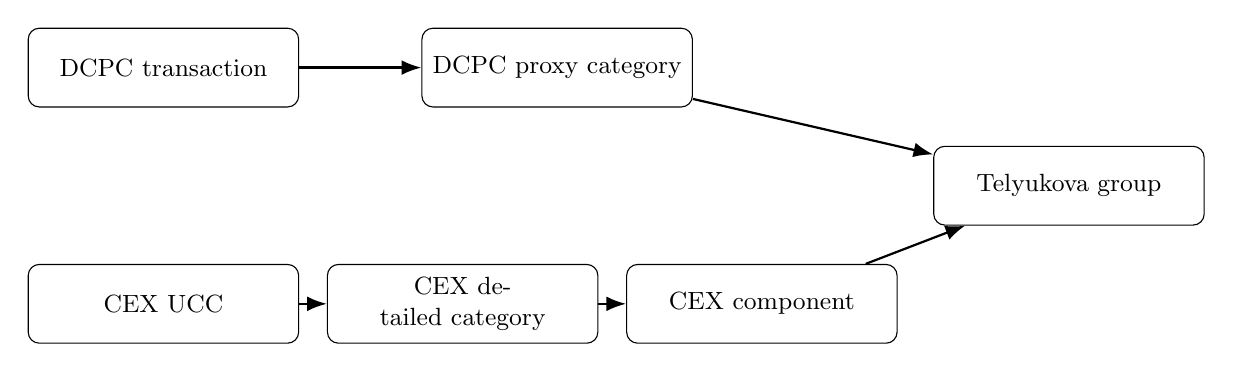
\begin{tikzpicture}
	[
	box/.style={
		draw,
		rounded corners,
		align=center,
		minimum height=10mm,
		text width=32mm,
		font=\small
	},
	arrow/.style={
		-{Latex[length=2.5mm]},
		thick
	}
	]
	
	% DCPC branch
	\node[box] (dcpc_transaction) at (0,1.5)
	{DCPC transaction};
	
	\node[box] (dcpc_category) at (5,1.5)
	{DCPC proxy category};
	
	% CEX branch
	\node[box] (cex_ucc) at (0,-1.5)
	{CEX UCC};
	
	\node[box] (cex_detail) at (3.8,-1.5)
	{CEX detailed category};
	
	\node[box] (cex_component) at (7.6,-1.5)
	{CEX component};
	
	% Shared aggregation level
	\node[box] (telyukova_group) at (11.5,0)
	{Telyukova group};
	
	% Arrows
	\draw[arrow] (dcpc_transaction) -- (dcpc_category);
	\draw[arrow] (dcpc_category) -- (telyukova_group);
	
	\draw[arrow] (cex_ucc) -- (cex_detail);
	\draw[arrow] (cex_detail) -- (cex_component);
	\draw[arrow] (cex_component) -- (telyukova_group);
	
\end{tikzpicture}

\clearpage

\begin{landscape}
	\footnotesize
	\setlength{\tabcolsep}{5pt}
	\renewcommand{\arraystretch}{1.25}
	
	\begin{longtable}{
			>{\RaggedRight\arraybackslash}p{0.20\linewidth}
			>{\RaggedRight\arraybackslash}p{0.31\linewidth}
			>{\RaggedRight\arraybackslash}p{0.41\linewidth}
		}
		\caption{Identification of DCPC proxy consumption categories}
		\label{tab:dcpc-category-identification}\\
		
		\toprule
		DCPC proxy category &
		Merchant code and meaning &
		Follow-up identification rule and meaning \\
		\midrule
		\endfirsthead
		
		\toprule
		DCPC proxy category &
		Merchant code and meaning &
		Follow-up identification rule and meaning \\
		\midrule
		\endhead
		
		\bottomrule
		\endfoot
		
		\code{food_grocery_proxy} &
		\code{merch}=1: Grocery stores, convenience stores without gas stations,
		and pharmacies. &
		None. The merchant code alone identifies the proxy category. \\
		
		\code{food_restaurant_bar_proxy} &
		\code{merch}=3: Sit-down restaurants and bars. &
		None. The merchant code alone identifies the proxy category. \\
		
		\code{food_fast_service_proxy} &
		\code{merch}=4: Fast-food restaurants, coffee shops, cafeterias, and
		food trucks. &
		None. The merchant code alone identifies the proxy category. \\
		
		\code{rent} &
		\code{merch}=14: Rent for apartments, homes, or other buildings,
		including payments to real-estate companies and property managers. &
		None. The merchant code alone identifies the category. \\
		
		\code{mortgage_payment} &
		\code{merch}=15: Financial-services providers, including mortgage
		companies, banks, credit-card companies, and insurance companies. &
		\code{pay010}=2: Purpose was to make a loan payment; and
		\code{pay011}=1: the loan was a mortgage. \\
		
		\code{utilities} &
		Either \code{merch}=8: Nongovernment utilities, including electricity,
		natural gas, water, sewer, trash, and heating oil; or
		\code{merch}=19: Government taxes or fees. &
		For \code{merch}=8, no follow-up is required.
		
		For \code{merch}=19:
		\code{pay040}=1 means a government purchase of goods or services, and
		\code{pay041}=1 identifies electricity, water, or sewer. \\
		
		\code{communications_entertainment_proxy} &
		\code{merch}=10: Telephone, internet, cable or satellite television,
		streaming services, and movie theaters. &
		None. The merchant code alone identifies the proxy category. \\
		
		\code{household_operations_bill_proxy} &
		\code{merch}=6: General services; or
		\code{merch}=11: Building contractors, plumbers, electricians, and
		HVAC providers. &
		\code{from_bill_section}=1: The transaction originated in the
		bill-reminder section. These records are assigned to household operations
		before the general contractor rule is evaluated. \\
		
		\code{household_repairs} &
		\code{merch}=11: Building contractors, plumbers, electricians, and
		HVAC providers. &
		No additional follow-up. This category contains the remaining
		\code{merch}=11 transactions after the bill-reminder household-operations
		rule has been applied. \\
		
		\code{homeowners_renters_insurance} &
		\code{merch}=15: Financial-services provider. &
		\code{pay010}=3: Purpose was to pay for insurance; and either
		\code{pay016}=1: homeowners insurance, or
		\code{pay016}=2: renters insurance. \\
		
		\code{property_taxes} &
		\code{merch}=19: Government taxes or fees. &
		\code{pay040}=2: Purpose was to pay taxes; and
		\code{pay042}=4: the tax was a property tax. \\
		
		\code{public_transport_tolls} &
		Either \code{merch}=21: Public transportation and tolls; or
		\code{merch}=19: Government taxes or fees. &
		For \code{merch}=21, no follow-up is required.
		
		For \code{merch}=19:
		\code{pay040}=1 means a government purchase of goods or services, and
		either \code{pay041}=5 identifies tolls or
		\code{pay041}=7 identifies public transportation. \\
		
		\code{taxi_air_delivery_proxy} &
		\code{merch}=9: Taxis, airplanes, and delivery services. &
		None. The merchant code alone identifies the proxy category. \\
		
		\code{health_insurance} &
		One of three merchant codes:
		\code{merch}=15, financial services;
		\code{merch}=18, medical-care providers; or
		\code{merch}=19, government. &
		Three alternative rules:
		
		(1) \code{merch}=15, \code{pay010}=3 for insurance, and
		\code{pay016}=3 for health insurance;
		
		(2) \code{merch}=18 and \code{pay030}=4, identifying the payee as an
		insurance company;
		
		(3) \code{merch}=19, \code{pay040}=1 for government goods or services,
		and \code{pay041}=8 for out-of-pocket health insurance, including
		Medicare supplemental insurance. \\
		
		\code{childcare} &
		Either \code{merch}=20: Schools, colleges, and childcare centers; or
		\code{merch}=19: Government taxes or fees. &
		For \code{merch}=20, \code{pay020}=3 identifies childcare.
		
		For \code{merch}=19, \code{pay040}=1 identifies government goods or
		services, and either \code{pay041}=3 identifies daycare or
		\code{pay041}=9 identifies childcare. \\
		
		\code{cash_contributions} &
		\code{merch}=17: Charitable or religious donations. &
		Either \code{pay050}=1: donation; or
		\code{pay050}=2: offering, tithe, or money placed in a collection plate. \\
		
	\end{longtable}
\end{landscape}

\subsection{Data Innovation Standard Deviation $\text{sd}(\eta_{it})$}

Table \ref{tab:liquidity-demand-innovation-volatility-2018-2019} reports $\widehat{\alpha}$ and $\operatorname{sd}(\widehat{\eta}_{it})$ from equations (\ref{eqn:telyukova_first_stage}) and (\ref{eqn:telyukova_second_stage}) using monthly CEX data from 2018--2019. We include the two aforementioned alternate definitions of $c^{liq}_{it}$ for sensitivity checks. Both stages and the reported innovation standard deviations are unweighted. 

\begin{table}[htbp]
	\centering
	\small
	\setlength{\tabcolsep}{8pt}
	\renewcommand{\arraystretch}{1.2}
	\caption{Monthly empirical innovation-volatility estimates, 2018--2019}
	\label{tab:liquidity-demand-innovation-volatility-2018-2019}
	\begin{tabular}{
			>{\RaggedRight\arraybackslash}p{0.39\textwidth}
			ccc
		}
		\toprule
		Liquid-consumption measure
		& $\widehat{\alpha}$
		& $\operatorname{sd}(\widehat{\eta}_{it})$
		& $\operatorname{sd}(\widehat{\eta}_{it})$ (\%) \\
		\midrule
		Benchmark
		& 0.141 & 0.271 & 27.14 \\
		Excluding food, alcohol, and tobacco
		& 0.139 & 0.285 & 28.53 \\
		Excluding food, alcohol, tobacco, and property taxes
		& 0.109 & 0.325 & 32.47 \\
		\bottomrule
	\end{tabular}
\end{table}

\subsection{Adjacent-month Liquid Consumption Correlation for Moment Matching}

The model persistence $\rho$ is calibrated by matching the correlation between liquid consumption in consecutive months. Table \ref{tab:adjacent-consumption-correlations-2019} reports the 2019 correlations in levels and logs. These are pooled, unweighted correlations across strictly consecutive months for which both consumer-unit observations have positive liquid consumption. 

\begin{table}[htbp]
	\centering
	\small
	\setlength{\tabcolsep}{6pt}
	\renewcommand{\arraystretch}{1.2}
	\caption{Adjacent-month liquid-consumption correlations, 2019}
	\label{tab:adjacent-consumption-correlations-2019}
	\resizebox{\textwidth}{!}{%
		\begin{tabular}{
				>{\RaggedRight\arraybackslash}p{0.34\textwidth}
				rrrr
			}
			\toprule
			Liquid-consumption measure
			& Adjacent pairs
			& Households
			& $\operatorname{Corr}(c_{it}^{liq},c_{i,t-1}^{liq})$
			& $\operatorname{Corr}(\log c_{it}^{liq},\log c_{i,t-1}^{liq})$ \\
			\midrule
			Benchmark
			& 51{,}095 & 11{,}432 & 0.589 & 0.852 \\
			Excluding food, alcohol, and tobacco
			& 50{,}951 & 11{,}397 & 0.560 & 0.844 \\
			Excluding food, alcohol, tobacco, and property taxes
			& 50{,}913 & 11{,}387 & 0.509 & 0.810 \\
			\bottomrule
		\end{tabular}%
	}
\end{table}

\end{document}	
